\section{Transport of Materials in Living Things} \index{Transport|textbf}

\begin{multicols}{2}


\section*{Diffusion} \index{Diffusion}


\subsection{Diffusion in Liquids}

\begin{center}
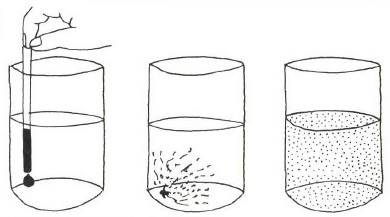
\includegraphics[width=0.4\textwidth]{./img/vso/diffusion.jpg}
\end{center}

\begin{description*}
%\item[Subtopic:]{}
\item[Materials:]{Plastic water bottle, food colour (liquid or powder)}
%\item[Setup:]{}
\item[Procedure:]{Put a drop or small amount of powdered food colour into the water without shaking and observe what happens.}
%\item[Hazards:]{}
%\item[Questions:]{}
\item[Observations:]{The colour gradually spreads throughout the water.}
\item[Theory:]{This spreading is due to the motion of the particles of food colour. This process is called \emph{diffusion}.}
\item[Applications:]{Organisms utilize diffusion to balance nutrient concentrations in cells and to transfer oxygen into the bloodstream during respiration.}
%\item[Notes:]{}
\end{description*}

\subsection{Smelling Particles}

\begin{description*}
%\item[Subtopic:]{}
\item[Materials:]{Orange or other citrus fruit, box}
%\item[Setup:]{}
\item[Procedure:]{Peel and orange and have students raise their hands when they begin to smell it. Now place a box in front of the orange and repeat the test.}
%\item[Hazards:]{}
%\item[Questions:]{}
\item[Observations:]{Students in the front center of the room should be the first to raise their hands, followed by those near the sides and in the back. When the orange is peeled behind the box it takes longer for the smell to reach the students.}
\item[Theory:]{Tiny particles from the orange peel spread by diffusion to students' noses. The box hinders the motion of the particles and so they reach the students more slowly.}
\item[Applications:]{Air fresheners and other sprays}
%\item[Notes:]{}
\end{description*}

%==================================================================================================%

\section*{Osmosis} \index{Osmosis}




\subsection{Semi-Permeable Membranes}

\begin{center}
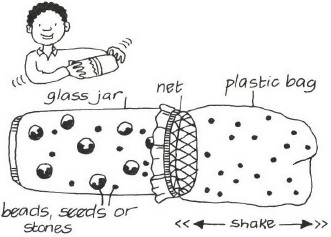
\includegraphics[width=0.4\textwidth]{./img/vso/membrane.jpg}
\end{center}

\begin{description*}
%\item[Subtopic:]{}
\item[Materials:]{Glass jar, clear plastic bag, small beads or stones, beans, netting, string/rubber band}
\item[Setup:]{Place the mixture of beads and beans in the jar. Place the net and plastic bag over the top and tie them on securely.}
\item[Procedure:]{Shake the apparatus for a few seconds.}
%\item[Hazards:]{}
%\item[Questions:]{}
\item[Observations:]{Only the small beads pass through the netting. The beans remain in the jar.}
\item[Theory:]{The beads represent small molecules and the net is a semi-permeable membrane. The beans are too large to pass through and hence remain in the jar.}
%\item[Applications:]{Water filters, organism cell membranes}
%\item[Notes:]{}
\end{description*}

\subsection{Osmosis in Dead and Living Tissues}

\begin{center}
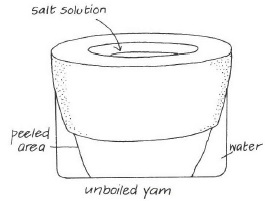
\includegraphics[width=0.35\textwidth]{./img/vso/osmosis-dead-living.jpg}
\end{center}

\begin{description*}
%\item[Subtopic:]{}
\item[Materials:]{Potato, knife, 2 dishes of water}
%\item[Setup:]{}
\item[Procedure:]{Cut the potato in half
and boil one piece. When it has
cooled, hollow out the centre of
both pieces and half fill
with the sugar solution.
Peel the lower half of both
pieces and then place each in a dish of water for an hour or so.}
%\item[Hazards:]{}
%\item[Questions:]{}
\item[Observations:]{Water will only enter the unboiled potato.}
\item[Theory:]{Boiling one potato kills its cells and so osmosis does not occur.}
%\item[Applications:]{}
%\item[Notes:]{}
\end{description*}

\columnbreak

\subsection{Vanilla Balloon}

\begin{center}
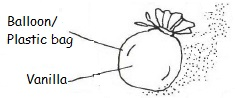
\includegraphics[width=0.35\textwidth]{./img/vso/osmosis-vanilla.jpg}
\end{center}

\begin{description*}
%\item[Subtopic:]{}
\item[Materials:]{Balloon/plastic bag, vanilla, straw/syringe}
%\item[Setup:]{}
\item[Procedure:]{Place a few drops of vanilla in a deflated balloon. Now blow up the balloon and tie it shut.}
%\item[Hazards:]{}
%\item[Questions:]{}
\item[Observations:]{You can smell the vanilla through the surface of the balloon.}
\item[Theory:]{The balloon acts as a \emph{semi-permeable membrane} which allows some of the vanilla particles to pass through and reach your nose. Other particles remain inside the balloon.}
%\item[Applications:]{}
%\item[Notes:]{}
\end{description*}

\subsection[Osmosis/Active Transport Model]{Osmosis/Active Transport \hfill \\ Model} \index{Active transport}% Source 79

\begin{center}
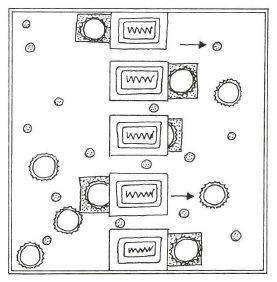
\includegraphics[width=0.45\textwidth]{./img/vso/active-transport.jpg}
\end{center}

\begin{description*}
%\item[Subtopic:]{}
\item[Materials:]{Cardboard tray, matchboxes, peas/beans, bottle caps, tape}
%\item[Setup:]{Tape the matchboxes to a tray. The gaps between them should allow small objects to pass (e.g. peas) but prevent
%movement of larger ones (soda bottle caps).}
\item[Setup:]{Tape the matchboxes to a tray, spaced as shown.}
\item[Procedure:]{Place ten soda caps and ten peas in one
side of the tray and twenty peas in the other side. Shake the tray gently. Count the
peas in each side.}
%\item[Hazards:]{}
%\item[Questions:]{}
%\item[Observations:]{}
\item[Theory:]{The
matchboxes represent a selectively
permeable membrane. The spaces
allow small objects through, but
not larger ones. The peas
represent water molecules which
move freely. The bottle caps
represent larger glucose
molecules which need to be
placed in the matchbox drawers
and actively pushed through to
the other side.}
%\item[Applications:]{}
%\item[Notes:]{}
\end{description*}

\columnbreak

\subsection{Potato Osmosis}

\begin{center}
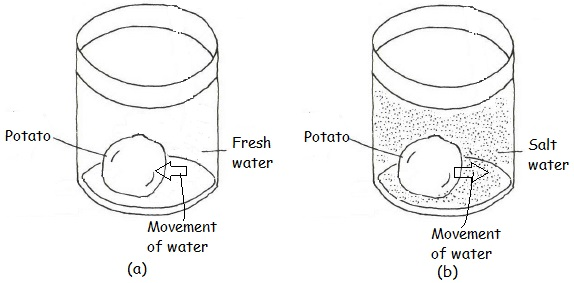
\includegraphics[width=0.49\textwidth]{./img/vso/osmosis-potato-full.jpg}
\end{center}

\begin{description*}
%\item[Subtopic:]{}
\item[Materials:]{Potato, 2 water bottles, salt, water}
\item[Setup:]{Cut two equal size pieces of potato. Fill one bottle with fresh water and the other with a salt water solution.}
\item[Procedure:]{Put one piece of potato in each bottle. Observe over the next few hours.}
%\item[Hazards:]{}
%\item[Questions:]{}
\item[Observations:]{The potato in fresh water swells while the potato in salt water shrivels up.}
\item[Theory:]{Through osmosis, water moves from a region of low concentration to one of high concentration through a semi-permeable membrane (the potato). In fresh water, the potato has the higher salt concentration, so water enters in order to make a balance. In salt water, the concentration of the surrounding water is higher than that of the potato, so water inside the potato moves outside to dilute the salt solution.}
%\item[Applications:]{}
%\item[Notes:]{Try this experiment again with a boiled potato. Do you observe any differences?}
\end{description*}

%\subsection{Osmosis with Eggs} % VSO 25
%
%\begin{center}
%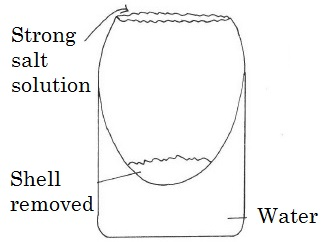
\includegraphics[width=0.4\textwidth]{./img/vso/osmosis-eggs.jpg}
%\end{center}
%
%\begin{description*}
%%\item[Subtopic:]{}
%\item[Materials:]{Empty eggshell, strong salt solution, jar of water}
%%\item[Setup:]{}
%\item[Procedure:]{Remove the hard outer shell at
%one end of the eggshell to
%expose the inner membrane. Half
%fill the egg with salt solution and
%place it in the jar so that the
%water level is above the exposed
%membrane and leave for a couple
%of hours. }
%%\item[Hazards:]{}
%\item[Observations:]{The level of
%the solution inside the egg rises,
%indicating water has crossed the
%membrane, i.e. osmosis has
%occurred.}
%%\item[Questions:]{What happens if you use sugar solution instead of salt? What if you put salt solution in the jar as well as the egg?}
%\item[Theory:]{Water travels from an area of low concentration to an area of high concentration of salts.}
%%\item[Applications:]{}
%%\item[Notes:]{}
%\end{description*}

\subsection{Guard Cells in Osmosis}

\begin{center}
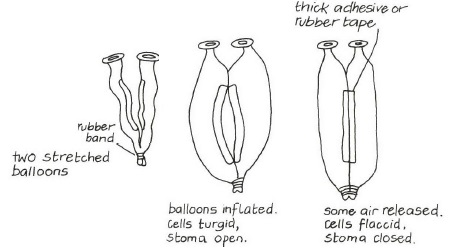
\includegraphics[width=0.49\textwidth]{./img/vso/osmosis-guard-cells.jpg}
\end{center}

\begin{description*}
%\item[Subtopic:]{}
\item[Materials:]{2 long balloons, tape, rubber band}
%\item[Setup:]{}
\item[Procedure:]{Stick the adhesive tape down one
side of each balloon as shown.
When the balloons are both fully
inflated (turgid) the `stoma' is
open. If you let out some of the
air, (the 'guard cells' become
flaccid), the `stoma' closes.}
%\item[Hazards:]{}
%\item[Questions:]{}
%\item[Observations:]{}
%\item[Theory:]{}
%\item[Applications:]{}
%\item[Notes:]{}
\end{description*}

\columnbreak

%==================================================================================================%

\section*{Transport in Mammals} \index{Transport! in mammals} \index{Mammals! transport in}

%==================================================================================================%

\section*{The Mammalian Heart}  \index{Heart}


\subsection{Heart Pump Action} % VSO 32

\begin{center}
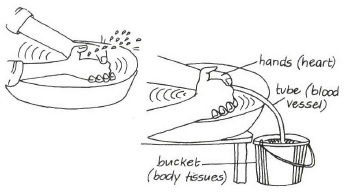
\includegraphics[width=0.49\textwidth]{./img/vso/heart-pump.jpg}
\end{center}

\begin{description*}
%\item[Subtopic:]{}
\item[Materials:]{2 bowls or buckets, rubber/plastic tubing}
%\item[Setup:]{}
\item[Procedure:]{Open and close your hands as
shown while they are in a bucket
or bowl of water. Now hold a
rubber tube as shown. Open and
close the palms again. }
%\item[Hazards:]{}
%\item[Questions:]{}
%\item[Observations:]{}
\item[Theory:]{The opening and closing of the palms represent the relaxation and contraction of the heart
muscles. Blood enters the chambers of the heart when the muscles relax and is forced out
into the vessels as they contract.}
%\item[Applications:]{}
%\item[Notes:]{}
\end{description*}

\subsection{Heart Model} % VSO 32

\begin{center}
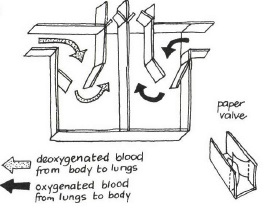
\includegraphics[width=0.45\textwidth]{./img/vso/heart-model.jpg}
\end{center}

\begin{description*}
%\item[Subtopic:]{}
\item[Materials:]{Cardboard box, paper}
%\item[Setup:]{}
\item[Procedure:]{Make a model of the heart from a
cardboard box as shown. Thin
paper is used for the valves.}
%\item[Hazards:]{}
%\item[Questions:]{}
%\item[Observations:]{}
\item[Theory:]{The heart is a four-chambered muscular organ. The upper chambers are thin-walled atria,
which receive blood from the veins. The lower two chambers are the thick-walled ventricles
which pump blood into arteries.}
%\item[Applications:]{}
%\item[Notes:]{}
\end{description*}

%==================================================================================================%

\section*{Blood Vessels} \index{Blood! vessels}

%==================================================================================================%

\subsection{Measuring Pulse} \index{Pulse rate}% VSO 32

\begin{center}
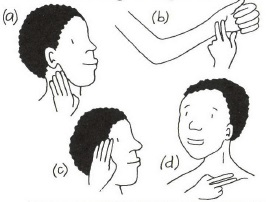
\includegraphics[width=0.4\textwidth]{./img/vso/measuring-pulse.jpg}
\end{center}

\begin{description*}
%\item[Subtopic:]{}
%\item[Materials:]{}
%\item[Setup:]{}
\item[Procedure:]{There are various places on the body where the pulse may be taken.
They are (a) under the ear beside the angle of the jaw, (b) at the wrists,
(c) at the temple, (d) behind the collar bone.
Ask students to find the pulse of a partner. If they have difficulty, they
should move their fingers around or apply a little more pressure.}
%\item[Hazards:]{}
%\item[Questions:]{}
%\item[Observations:]{}
%\item[Theory:]{}
\item[Applications:]{Students can compare a partner's pulse rate before and after exercise.}
%\item[Notes:]{}
\end{description*}

\subsection{Simple Stethoscope} % VSO 32

\begin{center}
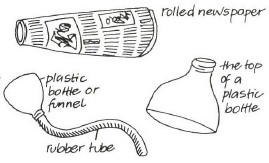
\includegraphics[width=0.45\textwidth]{./img/vso/stethoscope.jpg}
\end{center}

\begin{description*}
%\item[Subtopic:]{}
\item[Materials:]{Newspaper, plastic bottle, rubber tube}
%\item[Setup:]{}
\item[Procedure:]{Roll a newspaper up into a hollow tube. Place one end of tube against another students rib
cage (in the area of the heart).}
%\item[Hazards:]{}
%\item[Questions:]{}
\item[Observations:]{The heartbeat can be heard.}
%\item[Theory:]{}
\item[Applications:]{A doctor uses a stethoscope to focus the sound from the heart. Another stethoscope idea
could use funnels and plastic tube.}
%\item[Notes:]{}
\end{description*}

%\subsection{Looking at Blood Vessels} % VSO 33
%
%\begin{center}
%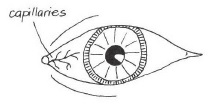
\includegraphics[width=0.4\textwidth]{./img/vso/blood-vessels-ex.jpg}
%\end{center}
%
%\begin{description*}
%%\item[Subtopic:]{}
%%\item[Materials:]{}
%%\item[Setup:]{}
%%\item[Procedure:]{}
%%\item[Hazards:]{}
%%\item[Questions:]{}
%\item[Observations:]{The blood capillaries in the corner
%of the eye clearly show capillary
%size. Red meat has so many tiny
%capillaries they give it its colour.}
%%\item[Theory:]{}
%%\item[Applications:]{}
%%\item[Notes:]{}
%\end{description*}

\subsection{Blood Vessel Model} % VSO 33

\begin{center}
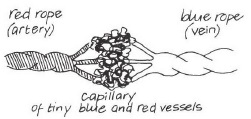
\includegraphics[width=0.4\textwidth]{./img/vso/blood-vessels.jpg}
\end{center}

\begin{description*}
%\item[Subtopic:]{}
\item[Materials:]{2 coloured ropes/strings (1 red, 1 blue)}
%\item[Setup:]{}
\item[Procedure:]{Untwist an end of each
rope until each end becomes a
mass of tiny thin strings. If you
twist the thin strings together
they form a mass of fine
capillaries.}
%\item[Hazards:]{}
%\item[Questions:]{}
%\item[Observations:]{}
%\item[Theory:]{}
%\item[Applications:]{}
%\item[Notes:]{}
\end{description*}

%==================================================================================================%

\section*{Blood} \index{Blood}

%==================================================================================================%

\subsection{Blood as a Transporter} % VSO 30

\begin{center}
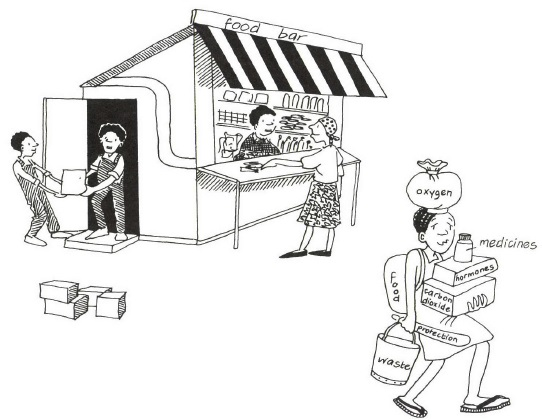
\includegraphics[width=0.49\textwidth]{./img/vso/blood-transport.jpg}
\end{center}

\begin{description*}
%\item[Subtopic:]{}
%\item[Materials:]{}
%\item[Setup:]{}
%\item[Procedure:]{}
%\item[Hazards:]{}
%\item[Observations:]{}
%\item[Theory:]{}
\item[Applications:]{Blood brings substances to the
cells, e.g. food and oxygen, and
removes others (waste and CO$_2$).
A food bar or shop has items
delivered, gives out items and
produces waste. This gives a good
analogy for the blood system.
Students can act out the role of
blood by picking up or putting
down items at different shops
(sites of the body).}
\item[Questions:]{Ask students what they pick up and put down at the following sites: lungs, liver, muscles, kidneys, etc.}
%\item[Notes:]{}
\end{description*}

\columnbreak

\subsection{Red and White Blood Cell Models} \index{Blood! cells} % VSO 30

\begin{center}
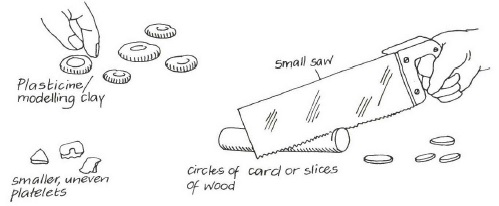
\includegraphics[width=0.49\textwidth]{./img/vso/red-white-model.jpg}
\end{center}

\begin{description*}
%\item[Subtopic:]{}
\item[Materials:]{Plasticine, clay or wooden rod, card or sponge}
\item[Setup:]{Red blood cells are biconcave discs with no nucleus. You can make
models from Plasticine or circles of wood. White blood cells could be
cut from thin sponge rubber sheet. They contain a nucleus which can
be drawn in on the sponge. Platelets, essential for clotting at open
wounds, can be made from smaller, irregular pieces of sponge, clay etc. }
\item[Procedure:]{Make red and white blood cells
by cutting shapes from cardboard,
paper or plastic.
Add platelets and then put
everything into water. Ask
students what the water
represents.}
%\item[Hazards:]{}
%\item[Questions:]{}
%\item[Observations:]{}
%\item[Theory:]{}
%\item[Applications:]{}
%\item[Notes:]{}
\end{description*}

\subsection{Engulfing Model} % VSO 31

\begin{center}
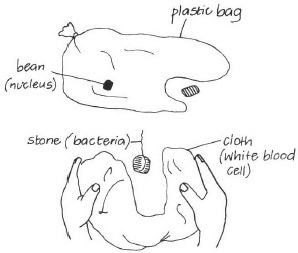
\includegraphics[width=0.49\textwidth]{./img/vso/engulfing.jpg}
\end{center}

\begin{description*}
%\item[Subtopic:]{}
\item[Materials:]{Clear plastic bag of water or cloth, stone or bean}
%\item[Setup:]{}
\item[Procedure:]{Partly fill a clear plastic bag with
water. Put a stone or bean inside
to represent the nucleus. By
shaping the bag, the action of a
white blood cell engulfing a
foreign body can be
demonstrated. You could use a
cloth, handkerchief or blanket as
a white blood cell. Shape the
cloth to show the pseudopodia
surrounding the foreign body.}
%\item[Hazards:]{}
%\item[Questions:]{}
%\item[Observations:]{}
%\item[Theory:]{}
%\item[Applications:]{}
%\item[Notes:]{}
\end{description*}

\columnbreak

\subsection{Germs and Antibodies} % Source 89

\begin{center}
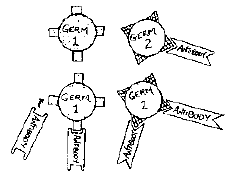
\includegraphics[width=0.45\textwidth]{./img/source/antibodies-2.png}
\end{center}

\begin{description*}
%\item[Subtopic:]{}
\item[Materials:]{Card, scissors}
%\item[Setup:]{}
\item[Procedure:]{Prepare circles of card with different shapes on their edges as shown in the diagram. The
circles represent the germ and the edge shapes their antigens. Now cut strips of card and
alter one end of each so it matches the edge shapes of the ``germ circles''.}
%\item[Hazards:]{}
%\item[Questions:]{}
%\item[Observations:]{}
\item[Theory:]{The strips of card represent the antibodies produced by the body to combat the antigens of
the germs. The antibodies will be able to act on a specific antigen.}
\item[Applications:]{}
%\item[Notes:]{}
\end{description*}

\subsection{Blood Clotting} % Source 86

\begin{center}
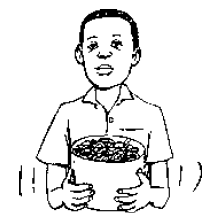
\includegraphics[width=0.3\textwidth]{./img/source/blood-clots.png}
\end{center}

\begin{description*}
%\item[Subtopic:]{}
\item[Materials:]{Red and white beans, container, grass or paper strips}
%\item[Setup:]{}
\item[Procedure:]{Place some red and white beans in a container to represent red and white blood cells.
Move them around by gently shaking. Mix thin strips of grass or paper with the beans and
repeat the shaking action. }
%\item[Hazards:]{}
%\item[Questions:]{}
\item[Observations:]{The beans are packed more securely by the strips.}
\item[Theory:]{The strips
represent the fibrin network }
%\item[Applications:]{}
%\item[Notes:]{}
\end{description*}

\columnbreak

\subsection{Transfusion Checkers} \index{Transfusion} % VSO 31

\begin{center}
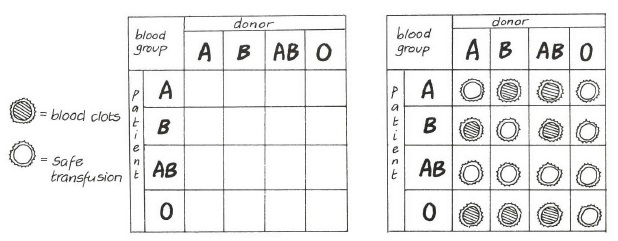
\includegraphics[width=0.49\textwidth]{./img/vso/transfusion-checkers.jpg}
\end{center}

\begin{description*}
%\item[Subtopic:]{}
\item[Materials:]{Bottle caps (2 types), card, coloured pens}
%\item[Setup:]{}
\item[Procedure:]{Draw out a base grid as shown. Use 2 types of bottle caps or counters to
show `safe' or `clot' transfusions.}
%\item[Hazards:]{}
\item[Questions:]{Can you place the tops on the right square to show which blood groups are compatible?
Which ones aren't?}
%\item[Observations:]{}
\item[Theory:]{The main red blood cells contain antigens, classified as blood groups A, B or AB. Blood
group O cells do not have antigens. Antibodies in plasma clump blood cells together.}
%\item[Applications:]{}
%\item[Notes:]{}
\end{description*}

\subsection{Transfusion Card Game}

\begin{center}
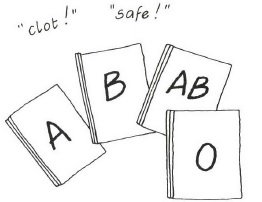
\includegraphics[width=0.4\textwidth]{./img/vso/transfusion-card.jpg}
\end{center}

\begin{description*}
%\item[Subtopic:]{}
\item[Materials:]{Cards, pen}
\item[Setup:]{Cut out 20 cards and label 5 for each blood group. }
\item[Procedure:]{Shuffle the cards and turn one card face up.
This is the patient's blood group. The next card turned over is the
donor's blood group. If a transfusion is possible, players must call `safe'.
If a transfusion would be dangerous they call `clot'. The first player to
call correctly wins the 2 cards. The player with the most cards wins the game.}
%\item[Hazards:]{}
%\item[Questions:]{}
%\item[Observations:]{}
%\item[Theory:]{}
%\item[Applications:]{}
%\item[Notes:]{}
\end{description*}

\columnbreak

%==================================================================================================%

\section*{Blood Circulation} \index{Blood! circulation}


\subsection{Circulation Game} % VSO 33
\label{sub:circulation-game}

\begin{center}
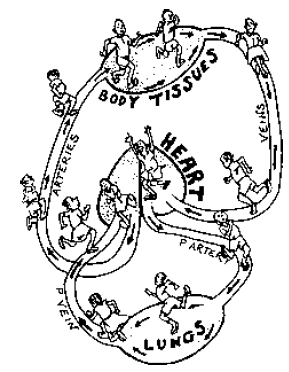
\includegraphics[width=0.49\textwidth]{./img/source/circulation-game.png}
%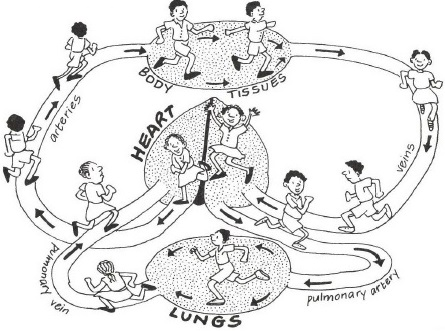
\includegraphics[width=0.49\textwidth]{./img/vso/circulation-game.jpg}
\end{center}

\begin{description*}
%\item[Subtopic:]{}
\item[Materials:]{String or chalk, red and blue flowers/papers, students}
\item[Setup:]{Mark out a model of the circulatory system on the ground using stones, string or chalk. Put
pieces of red flowers or paper in the area marked lungs and pieces of blue flowers or paper in
the area marked body tissues. }
\item[Procedure:]{To begin the game two or three pupils pick up blue petals at
the body tissues and follow the arrows through to the heart and on to the lungs. At the lungs
the pupils drop the blue flowers and pick up the red and return to the body tissues via the
other side of the heart.}
%\item[Hazards:]{}
%\item[Questions:]{}
\item[Observations:]{The pupils represent the flow of blood in the body. They must go through the heart twice
before completing the cycle of double circulation. }
\item[Theory:]{As blood flows it transports substances
such as oxygen (red flowers), carbon dioxide (blue flowers) and food materials. Pupils can
also act as heart valves.}
%\item[Applications:]{}
%\item[Notes:]{}
\end{description*}

%==================================================================================================%

\section*{Transport in Plants} \index{Plants! transport in} \index{Transport! in plants}


\subsection{Xylem and Phloem Game} \index{Xylem} \index{Phloem} % VSO 41

\begin{center}
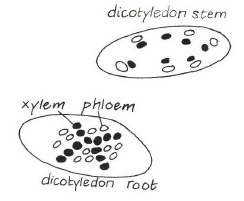
\includegraphics[width=0.4\textwidth]{./img/vso/xylem-phloem.jpg}
\end{center}

\begin{description*}
%\item[Subtopic:]{}
\item[Materials:]{Chalk, card/paper, coloured markers}
%\item[Setup:]{}
\item[Procedure:]{Chalk 2 circles on the floor or
table. Cut out 20 discs from card
or paper. Colour 10 to represent
xylem vessels and 10 to represent
phloem tubes. Use the discs
to show the arrangement of
vascular tissue in a root and a
dicotyledon stem.}
%\item[Hazards:]{}
\item[Questions:]{What are the differences in arrangement between stem and root?}
%\item[Observations:]{}
\item[Theory:]{Vascular tissue forms a ring of bundles in the stem but a central column in the root.}
%\item[Applications:]{}
%\item[Notes:]{}
\end{description*}

\subsection{Root Hairs} % Source 98

\begin{center}
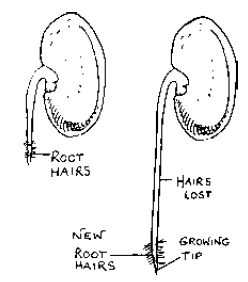
\includegraphics[width=0.3\textwidth]{./img/source/root-hairs.png}
\end{center}

\begin{description*}
%\item[Subtopic:]{}
\item[Materials:]{Pea/bean seeds, damp cloth}
%\item[Setup:]{}
\item[Procedure:]{Germinate some peas or bean seeds on a damp cloth or newspaper. Leave them until the
young root emerges. Observe the root tip using a hand lens if necessary.}
%\item[Hazards:]{}
%\item[Questions:]{}
\item[Observations:]{A fine covering of thin hair-like structures can be seen, just behind the root tip.}
\item[Theory:]{A root develops hairs just behind the growing tip. As the root gets older and larger the root
hairs are lost. Root hairs increase the surface area of the root for absorption of water and
mineral salts.}
%\item[Applications:]{}
%\item[Notes:]{}
\end{description*}

%\subsection{Capillarity}
%\begin{description*}
%%\item[Subtopic:]{}
%\item[Materials:]{Clear thin plastic straws with different diameters, shallow container (bottom of a water bottle/jar cap), various liquids, e.g. water, spirit and cooking oil}
%%\item[Setup:]{}
%\item[Procedure:]{Place one end of a straw into a container of water 1 cm deep so that the end is submerged but not touching the bottom. Mark the change in water level in the straw after about a minute. Repeat for different liquids and different size straws.}
%%\item[Hazards:]{}
%\item[Questions:]{Which liquid rises the farthest up the straw? Do liquids rise faster in wide or thin straws?}
%\item[Observations:]{The spirit rises to the greatest height while water rises the least. Liquids rise faster in thin straws compared to thick ones.}
%\item[Theory:]{Capillary rise results from adhesion, allowing the liquid to climb along the surface of the tube, as well as cohesion, which pulls the remainder of the liquid up. In a thin container, a larger proportion of liquid is attached to the side of the tube and a smaller proportion is being held by surface tension, so the adhesive force is strong enough to pull all the liquid up the tube.}
%%\item[Applications:]{}
%%\item[Notes:]{}
%\end{description*}

\columnbreak

\subsection{Capillary Rise} \index{Capillarity}

\begin{center}
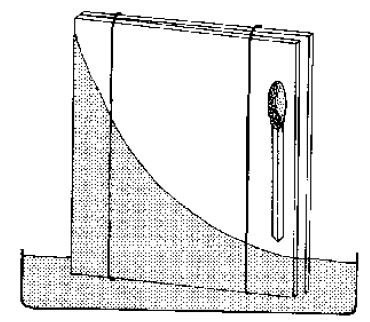
\includegraphics[width=0.4\textwidth]{./img/source/capillary-glass.jpg}
\end{center}

\begin{description*}
%\item[Subtopic:]{}
\item[Materials:]{2 glass sheets, match, rubber bands, water, food colour (optional)}
%\item[Setup:]{}
\item[Procedure:]{With the help of a rubber band and a matchstick, arrange two clean glass sheets as shown
in the diagram. Place the arrangement in a plate containing some water.}
%\item[Hazards:]{}
%\item[Questions:]{}
\item[Observations:]{Water rises to different heights along and between the glass sheets. }
\item[Theory:]{This is capillary
action. Capillary rise results from adhesion, allowing the liquid to climb along the surface of the glass, as well as cohesion, which pulls the remainder of the liquid up. Water rises more where the glass sheets are closer together.}
%\item[Applications:]{}
%\item[Notes:]{}
\end{description*}

%\subsection{Capillary Rise}
%
%\begin{center}
%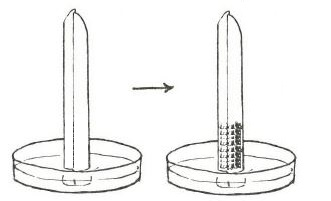
\includegraphics[width=0.4\textwidth]{./img/source/capillary-rise.jpg}
%\end{center}
%
%\begin{description*}
%%\item[Subtopic:]{}
%\item[Materials:]{Straws/chalk of different sizes, bottle, food colour, various liquids, e.g. water, spirit, kerosene, cooking oil}
%\item[Setup:]{Cut the bottom of a bottle to make a small dish.}
%\item[Procedure:]{Place one end of a straw/chalk into a dish of water 1 cm deep. Mark the change in level of the food colour after about a minute. Repeat for different liquids and different size straws.}
%%\item[Hazards:]{}
%\item[Questions:]{Which liquid rises the farthest up the straw? Do liquids rise faster in wide or thin straws?}
%\item[Observations:]{The spirit rises to the greatest height while water rises the least. Liquids rise faster in thin straws compared to thick ones.}
%\item[Theory:]{%Capillary rise results from adhesion, allowing the liquid to climb along the surface of the tube, as well as cohesion, which pulls the remainder of the liquid up. 
%In a thin container, a larger proportion of liquid is attached to the side of the tube and a smaller proportion is being held by surface tension, so the adhesive force is strong enough to pull more liquid up the tube.}
%%\item[Applications:]{}
%%\item[Notes:]{}
%\end{description*}

%\subsection{Moving Matches}
%
%%\begin{center}
%%\includegraphics[width=0.4\textwidth]{./img/.png}
%%\end{center}
%
%\begin{description*}
%%\item[Subtopic:]{}
%\item[Materials:]{Matches, water, straw, plastic lid}
%%\item[Setup:]{}
%\item[Procedure:]{Break several matches near the middle, but not so that they come apart. They should make acute angles. Place them on the plastic lid and place a few drops of water on the broken joints of the matches using the straw.}
%%\item[Hazards:]{}
%%\item[Questions:]{}
%\item[Observations:]{The matches close and return to their original straight shape.}
%\item[Theory:]{Water gets absorbed in the wooden matchstick and causes it to expand.}
%\item[Applications:]{This is why it is difficult to open a wooden door after it rains. The water rises up the wood causing it to expand into its frame.}
%%\item[Notes:]{}
%\end{description*}
%
%\columnbreak

%\subsection{Measuring Capillary Rise}
%
%\begin{center}
%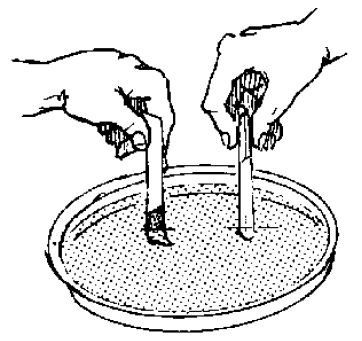
\includegraphics[width=0.4\textwidth]{./img/source/capillary-rise-meas.jpg}
%\end{center}
%
%\begin{description*}
%%\item[Subtopic:]{}
%\item[Materials:]{Paper, chalk, small dish/lid, water, food colour}
%\item[Setup:]{Cut off the bottom of a plastic bottle to make a water dish.}
%\item[Procedure:]{Place a strip of paper and a piece of chalk in a dish containing water. Leave the objects for some time and measure the rise in colour of each using a ruler.}
%%\item[Hazards:]{}
%%\item[Questions:]{}
%\item[Observations:]{The water rises faster in the chalk than in the paper.}
%\item[Theory:]{Chalk has smaller capillaries than paper, which allows water to rise faster.}
%%\item[Applications:]{}
%%\item[Notes:]{}
%\end{description*}

\subsection{Automatic Irrigation} \index{Irrigation}

\begin{center}
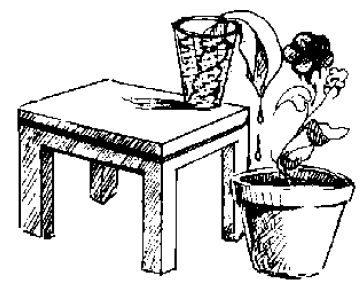
\includegraphics[width=0.3\textwidth]{./img/source/irrigation.png}
\end{center}

\begin{description*}
%\item[Subtopic:]{}
%\item[Materials:]{}
%\item[Setup:]{}
%\item[Procedure:]{}
%\item[Hazards:]{}
%\item[Questions:]{}
%\item[Observations:]{}
%\item[Theory:]{}
\item[Applications:]{Capillary action can be used to provide automatic irrigation for plants. Students can perform irrigation by dipping a porous material such as paper or cotton cloth in water.}
%\item[Notes:]{}
\end{description*}

\subsection{Water Movement in Plants} % VSO 41

\begin{center}
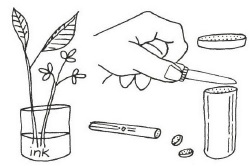
\includegraphics[width=0.4\textwidth]{./img/vso/water-movement.jpg}
\end{center}

\begin{description*}
%\item[Subtopic:]{}
\item[Materials:]{Various plant stems, food colour/ink (not black), water, knife}
%\item[Setup:]{}
\item[Procedure:]{Place a variety of different types of plants in coloured ink or dye and
leave them for a few hours. Slice off sections of the stem with a sharp
knife and examine them under a hand lens. }
%\item[Hazards:]{}
%\item[Questions:]{}
\item[Observations:]{The colour is located in the
xylem vessels which shows water is transported in the xylem. Some very young plants, such as
Balsam, are so transparent that
you can see the colour move up
the stem.}
%\item[Theory:]{}
%\item[Applications:]{}
%\item[Notes:]{}
\end{description*}

\subsection{Transpiration} \index{Transpiration} % VSO 40

\begin{center}
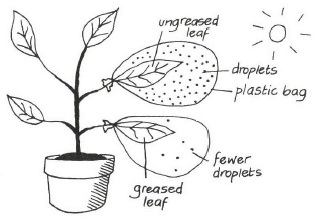
\includegraphics[width=0.4\textwidth]{./img/vso/transpiration.jpg}
\end{center}

\begin{description*}
%\item[Subtopic:]{}
\item[Materials:]{Potted plant, 2 small plastic bags, string, grease/Vaseline}
%\item[Setup:]{}
\item[Procedure:]{Place a polythene bag over the leaf of a living plant. Secure the bag to the stem with a
thread. Repeat the experiment with a greased leaf of the same size.}
%\item[Hazards:]{}
%\item[Questions:]{}
\item[Observations:]{Water droplets appear on the inside of the bag placed over the ungreased leaf. Very little
or no water collects in the other bag.}
\item[Theory:]{Water, which is absorbed from the soil by the plant, is lost through the pores (stomata) of the leaf. This is transpiration. There is no water loss from the greased leaf because the
grease blocks the pores.}
%\item[Applications:]{}
%\item[Notes:]{}
\end{description*}

%==================================================================================================%


\end{multicols}

\pagebreak